\documentclass[aspectratio=169,xcolor=table]{beamer}
\usepackage{epstopdf}
\usepackage{textgreek}
\usepackage{physics}
\usepackage{appendixnumberbeamer}
\usepackage{multicol}
\usepackage{pbox}
\usepackage{amssymb}
\usepackage{xcolor}
\usepackage{blindtext}
\usepackage{color, colortbl}
\usepackage{xspace}
\usepackage{listings}
\usepackage{tikz}
\usepackage{variable_defs}
\usetheme{NIU}
\usepackage{graphicx}
\graphicspath{{/Users/eparrish/Work/thesis/}}
\usepackage[style=ieee]{biblatex}
\setbeamertemplate{bibliography item}{\insertbiblabel}
\addbibresource{biblio.bib}
\usepackage{caption}
\captionsetup[figure]{labelformat=empty}% redefines the caption setup of the figures environment in the beamer class.

% \bibliography{biblio.bib}

% suppress navigation bar
\beamertemplatenavigationsymbolsempty

% Title
\title[Search for \HpmLong with ATLAS]
{Search for Charged Higgs Bosons in the \taulep Final State with \LUMI of \pp Collision Data at \sqs with the ATLAS Experiment}

% Sub Title
\subtitle{Dissertation Defense}

% Author
\author[Elliot Parrish]
{\texorpdfstring{\underline{Elliot Parrish}}{Elliot Parrish}}
\hypersetup{pdfauthor={Elliot Parrish}}

% - Give the names in the same order as the appear in the paper.
% - Use \and to separate authors name
% - Use the \inst{?} command only if the authors have different affiliation.

\institute[NIU] {\inst{\dag}Northern Illinois University, USA}
% \institute[IFJ PAN] {}
% - Use the \inst command only if there are several affiliations.
% - Keep it simple, no one is interested in your street address.

\date{October 13, 2022}
% \subject{} % only for pdf info

% if you want to disable section, subsection title page display, uncomment accordingly 
\AtBeginSection[]{
  \begin{frame}
  \vfill
  \centering
  \begin{beamercolorbox}[sep=8pt,center,shadow=true,rounded=true]{title}
    \usebeamerfont{title}\insertsectionhead\par%
  \end{beamercolorbox}
  \vfill
  \end{frame}
}
\AtBeginSubsection{}

% Title Graphics add befor titlepage
\titlegraphic{
\includegraphics[height=2.5cm]{NIU_logo.eps}}

\newcommand{\specialcell}[2][l]{%
  \begin{tabular}[#1]{@{}l@{}}#2\end{tabular}}

\newcommand{\Cross}{$\mathbin{\tikz [x=1.4ex,y=1.4ex,line width=.2ex, red] \draw (0,0) -- (1,1) (0,1) -- (1,0);}$}%
% \newcommand{\Hp}{\ensuremath{H^{\pm}}\xspace}
% \newcommand{\Etm}{\ensuremath{E_\text{T}^\text{miss}}\xspace}
% \newcommand{\pt}{\ensuremath{p_\text{T}}\xspace}
% \newcommand{\HpmLong}{\ensuremath{\Hp \rightarrow \tau \nu}\xspace}

\begin{document}
\frame{\titlepage}

% add logo after title page, so it does show on title page
\logo{
\includegraphics[trim=1cm 2.5cm 1cm 0,clip,width=1.3cm,keepaspectratio=true]{NIU_logo.eps}}
% \logo{\includegaraphics}


% Table of Contents
% \begin{frame}<beamer>{Table of Contents}
%     \tableofcontents
% \end{frame}

\begin{frame}{\contentsname}
  \begin{multicols}{2}
    \tableofcontents
  \end{multicols}
\end{frame}

\section{Introduction }
  
  \begin{frame}[t]{Welcome}
    \begin{itemize}
      \item This defense will take $\sim 1$ hour
      \begin{itemize}
        \item I will walk you through the work that is contained in my PhD dissertation
        \item After the presentation is complete, the committee and I will address comments privately
        \item When we are done, I will return, the committee will discuss among themselves then return
      \end{itemize}
      \item General Guidelines
      \begin{itemize}
        \item Please remain muted unless you are speaking
        \item There will be time at the end for questions, but feel free to interrupt if there is something urgent
      \end{itemize}
      \item Thank you for attending!
    \end{itemize}
  \end{frame}

\section{Theory }
  
  \subsection{The Standard Model }
  \begin{frame}[t]{What are we made of?}
    \begin{columns}
    \column{.59\textwidth}
      \begin{itemize}
        \item The scientific field of particle physics seeks to explain the building blocks of the universe
        \begin{itemize}
          \item How many fundamental particles are there?
          \item How do they interact with each other
        \end{itemize}
        \item The Standard Model of Particle Physics (SM)
        \begin{itemize}
          \item Matter is comprised of fermions
            \begin{itemize}
              \item Half-integer spin $(s=\frac{1}{2},\frac{3}{2},\frac{5}{2},etc.)$
              \item Anti-matter is identical to matter except for opposite electromagnetic charge
            \end{itemize}
          \item Forces are carried by an exchange of bosons
            \begin{itemize}
              \item Integer spin $(s=0,1,2,etc.)$
              \item Gluon (g) $\to$ Strong force
              \item Photon ($\gamma$) $\to$ Electromagnetism
              \item $W^{\pm},Z^{0}$ $\to$ Weak force
              % \item Higgs (H) $\to$ mass
            \end{itemize}
        \end{itemize}
      \end{itemize}
    \column{.4\textwidth}
      \begin{figure}
        \centering
        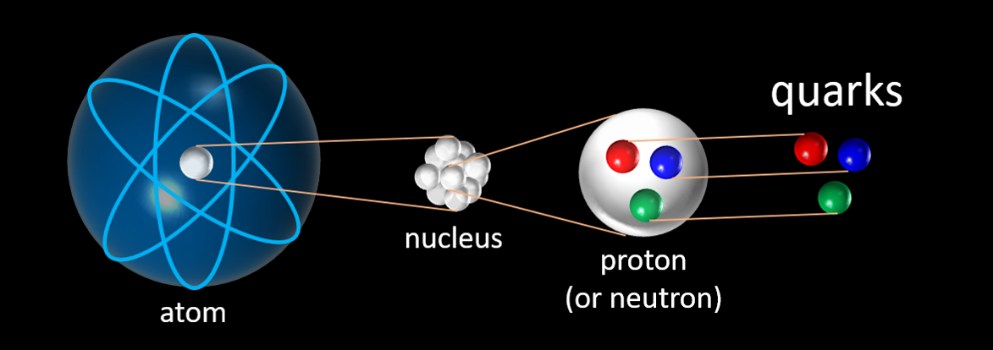
\includegraphics[width=\textwidth,keepaspectratio=true]{/Users/eparrish/Work/thesis/chapters/chapter2_theory/images/Atom_to_Quark_Cartoon.png}
        \caption{\tiny\cite{atom-to-quark}}
        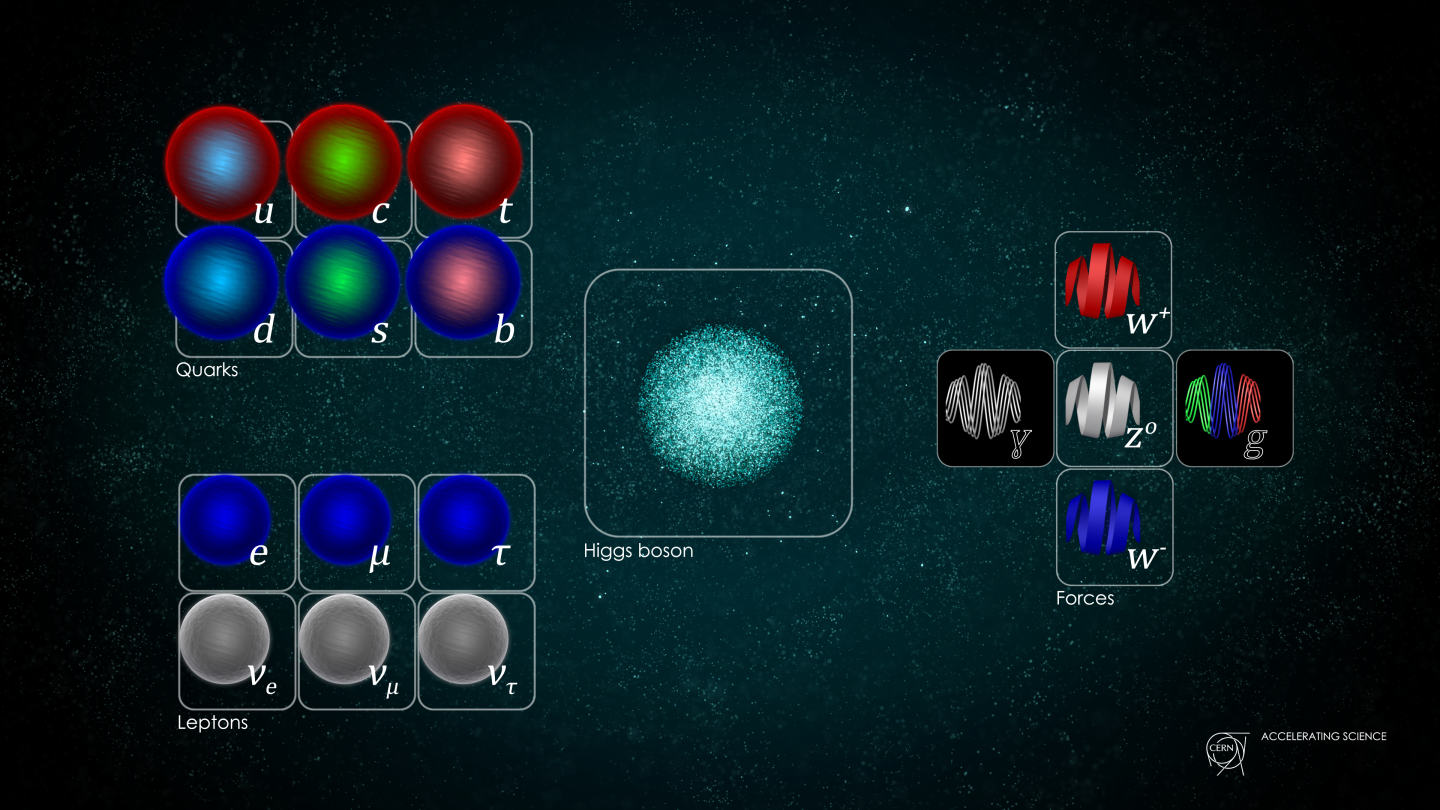
\includegraphics[width=\textwidth,keepaspectratio=true]{STDM higgs and field D.png}
      \end{figure}
    \end{columns}
  \end{frame}

  \subsection{Higgs Mechanism}

  \begin{frame}[t]{The Higgs Mechanism}
    \begin{columns}
    \column{.75\textwidth}
      \begin{itemize}
        \item Theorized by Higgs, Englert, and Brout in 1964
          \begin{itemize}
            \item Complex scalar doublet ($s=0$)
            \item Non-zero vacuum expectation value
          \end{itemize}
        \item Interactions with Higgs field give particles mass
        \item Discovered jointly by the ATLAS and CMS collaborations in 2012
      \end{itemize}
    \column{.25\textwidth}
      \begin{figure}
        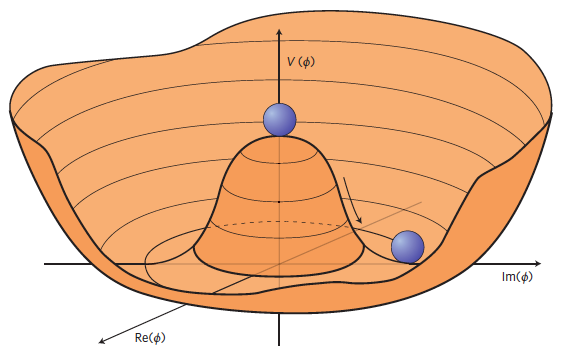
\includegraphics[width=.75\textwidth,keepaspectratio=true]{/Users/eparrish/Work/thesis/chapters/chapter2_theory/images/higgspotential.png}
        \caption{\tiny Higgs potential \cite{Higgs-phys}}
      \end{figure}
      \vspace{-.80cm}
      \begin{figure}
        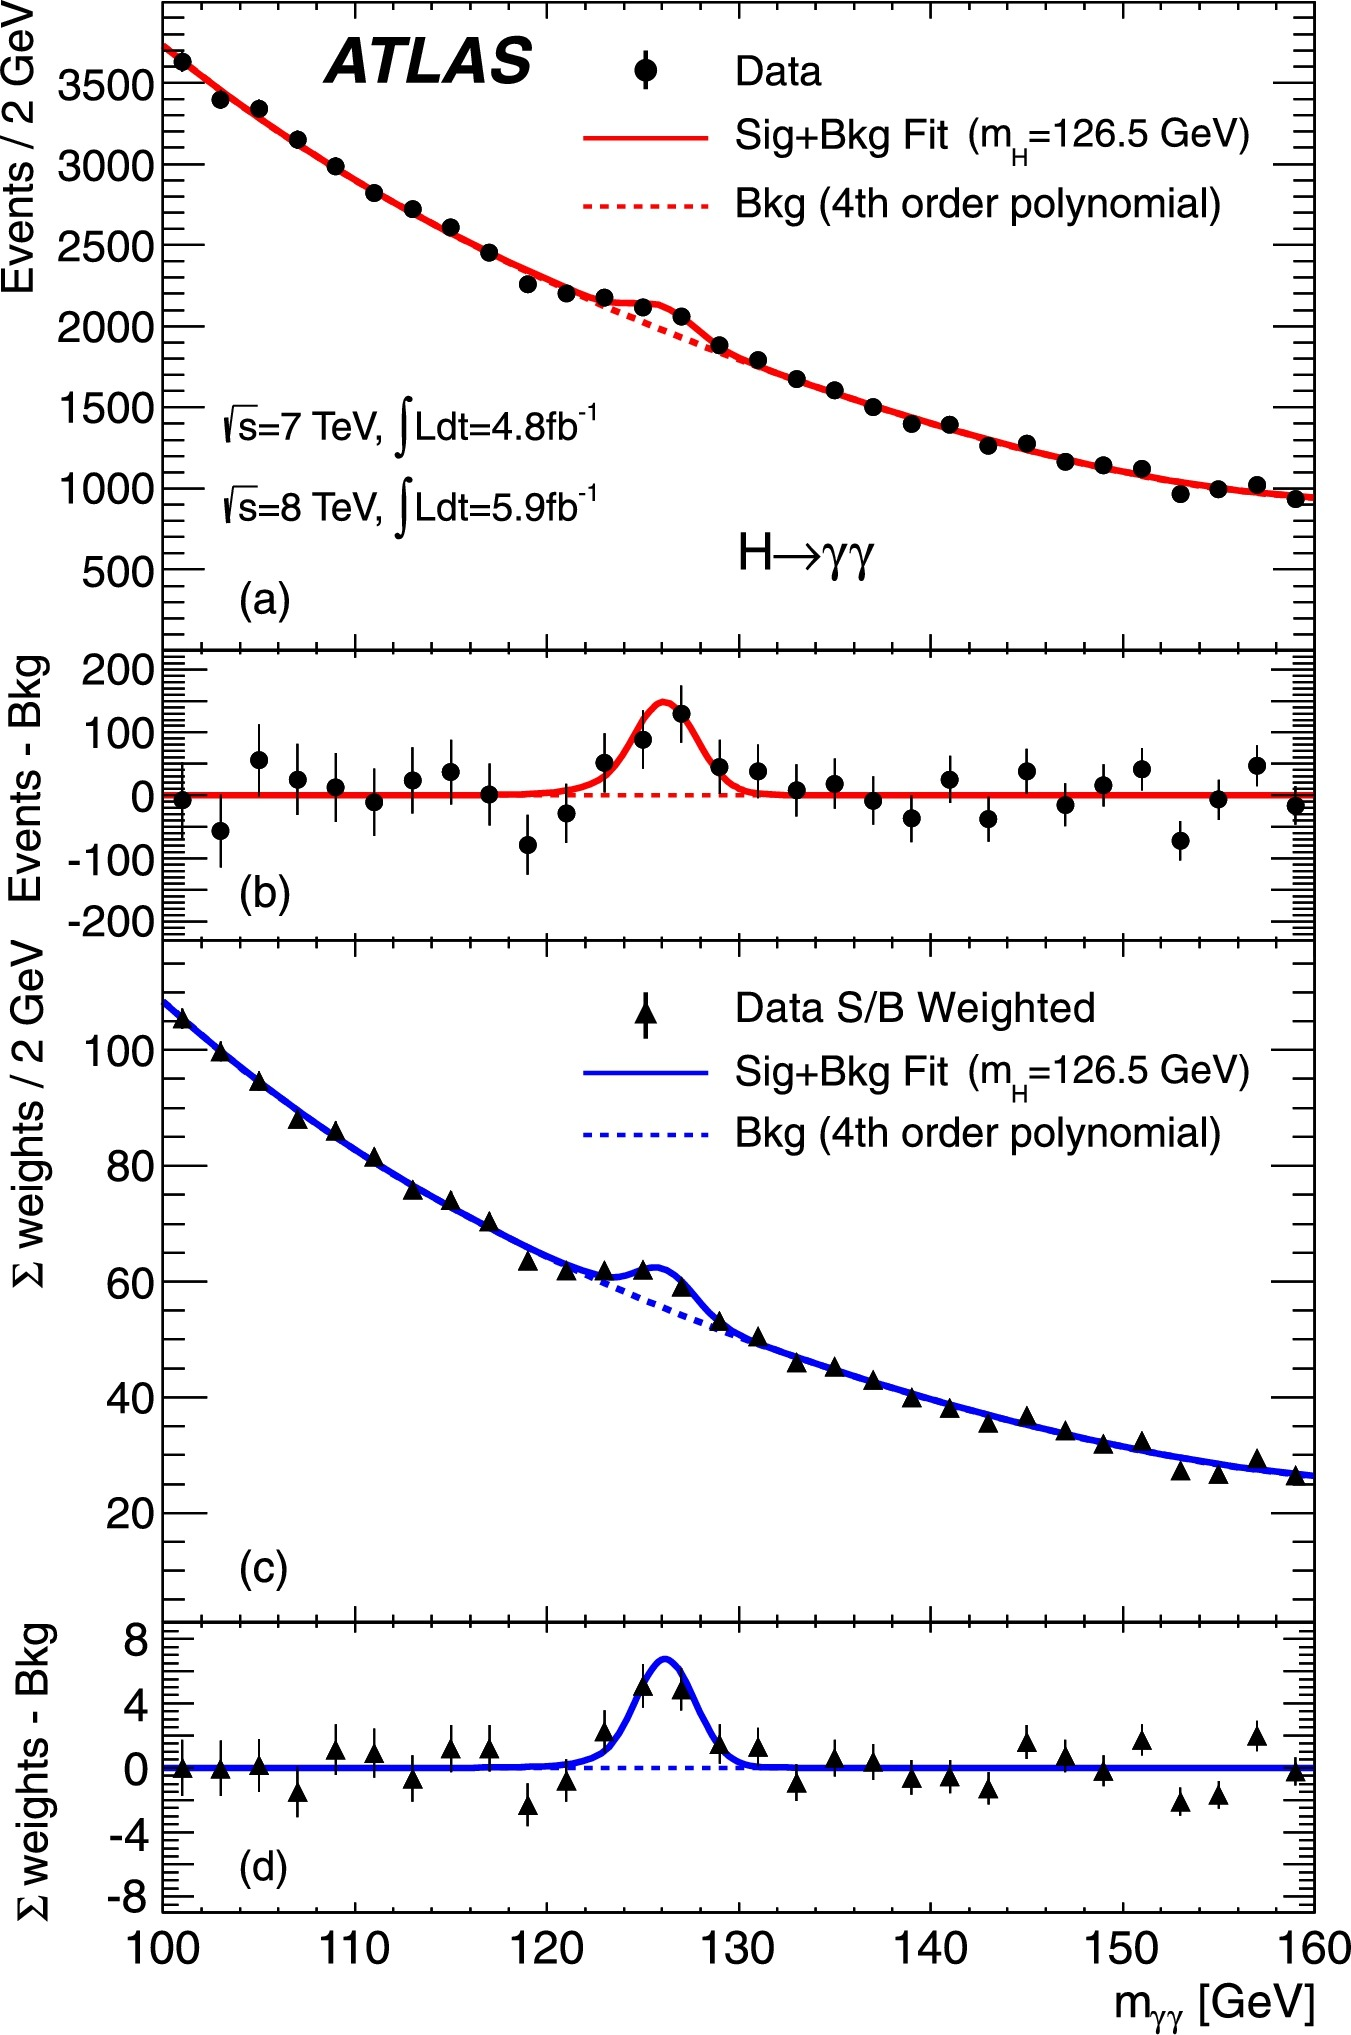
\includegraphics[height=.45\textheight,keepaspectratio=true]{/Users/eparrish/Work/thesis/chapters/chapter2_theory/images/Higgs_Discovery_gam_gam.jpeg}
        \caption{\tiny Higgs discovery \cite{higgs-discovery-atlas}}
      \end{figure}
    \end{columns}
  \end{frame}

  \begin{frame}[c]{The Standard Model}
    \begin{columns}
    \column{.45\textwidth}
      \small
      \begin{itemize}
        % \item Quantum field theory that explains the fundamental forces, particles, and their interactions
        \item Predicts the probabilities of particles decaying to others (among many other things)
        \begin{itemize}
          \item Has been thoroughly tested
          \item Measurements agree to a high degree of accuracy
        \end{itemize}
        \item Not a complete theory
        \begin{itemize}
          \item Gravity
          \item Matter-antimatter asymmetry in the universe
          \item Predicted neutrino masses are 0
          \begin{itemize}
            \item Observed neutrino mixing says otherwise
          \end{itemize}
        \end{itemize}
      \end{itemize}
    \column{.55\textwidth}
      \begin{figure}
        \centering
        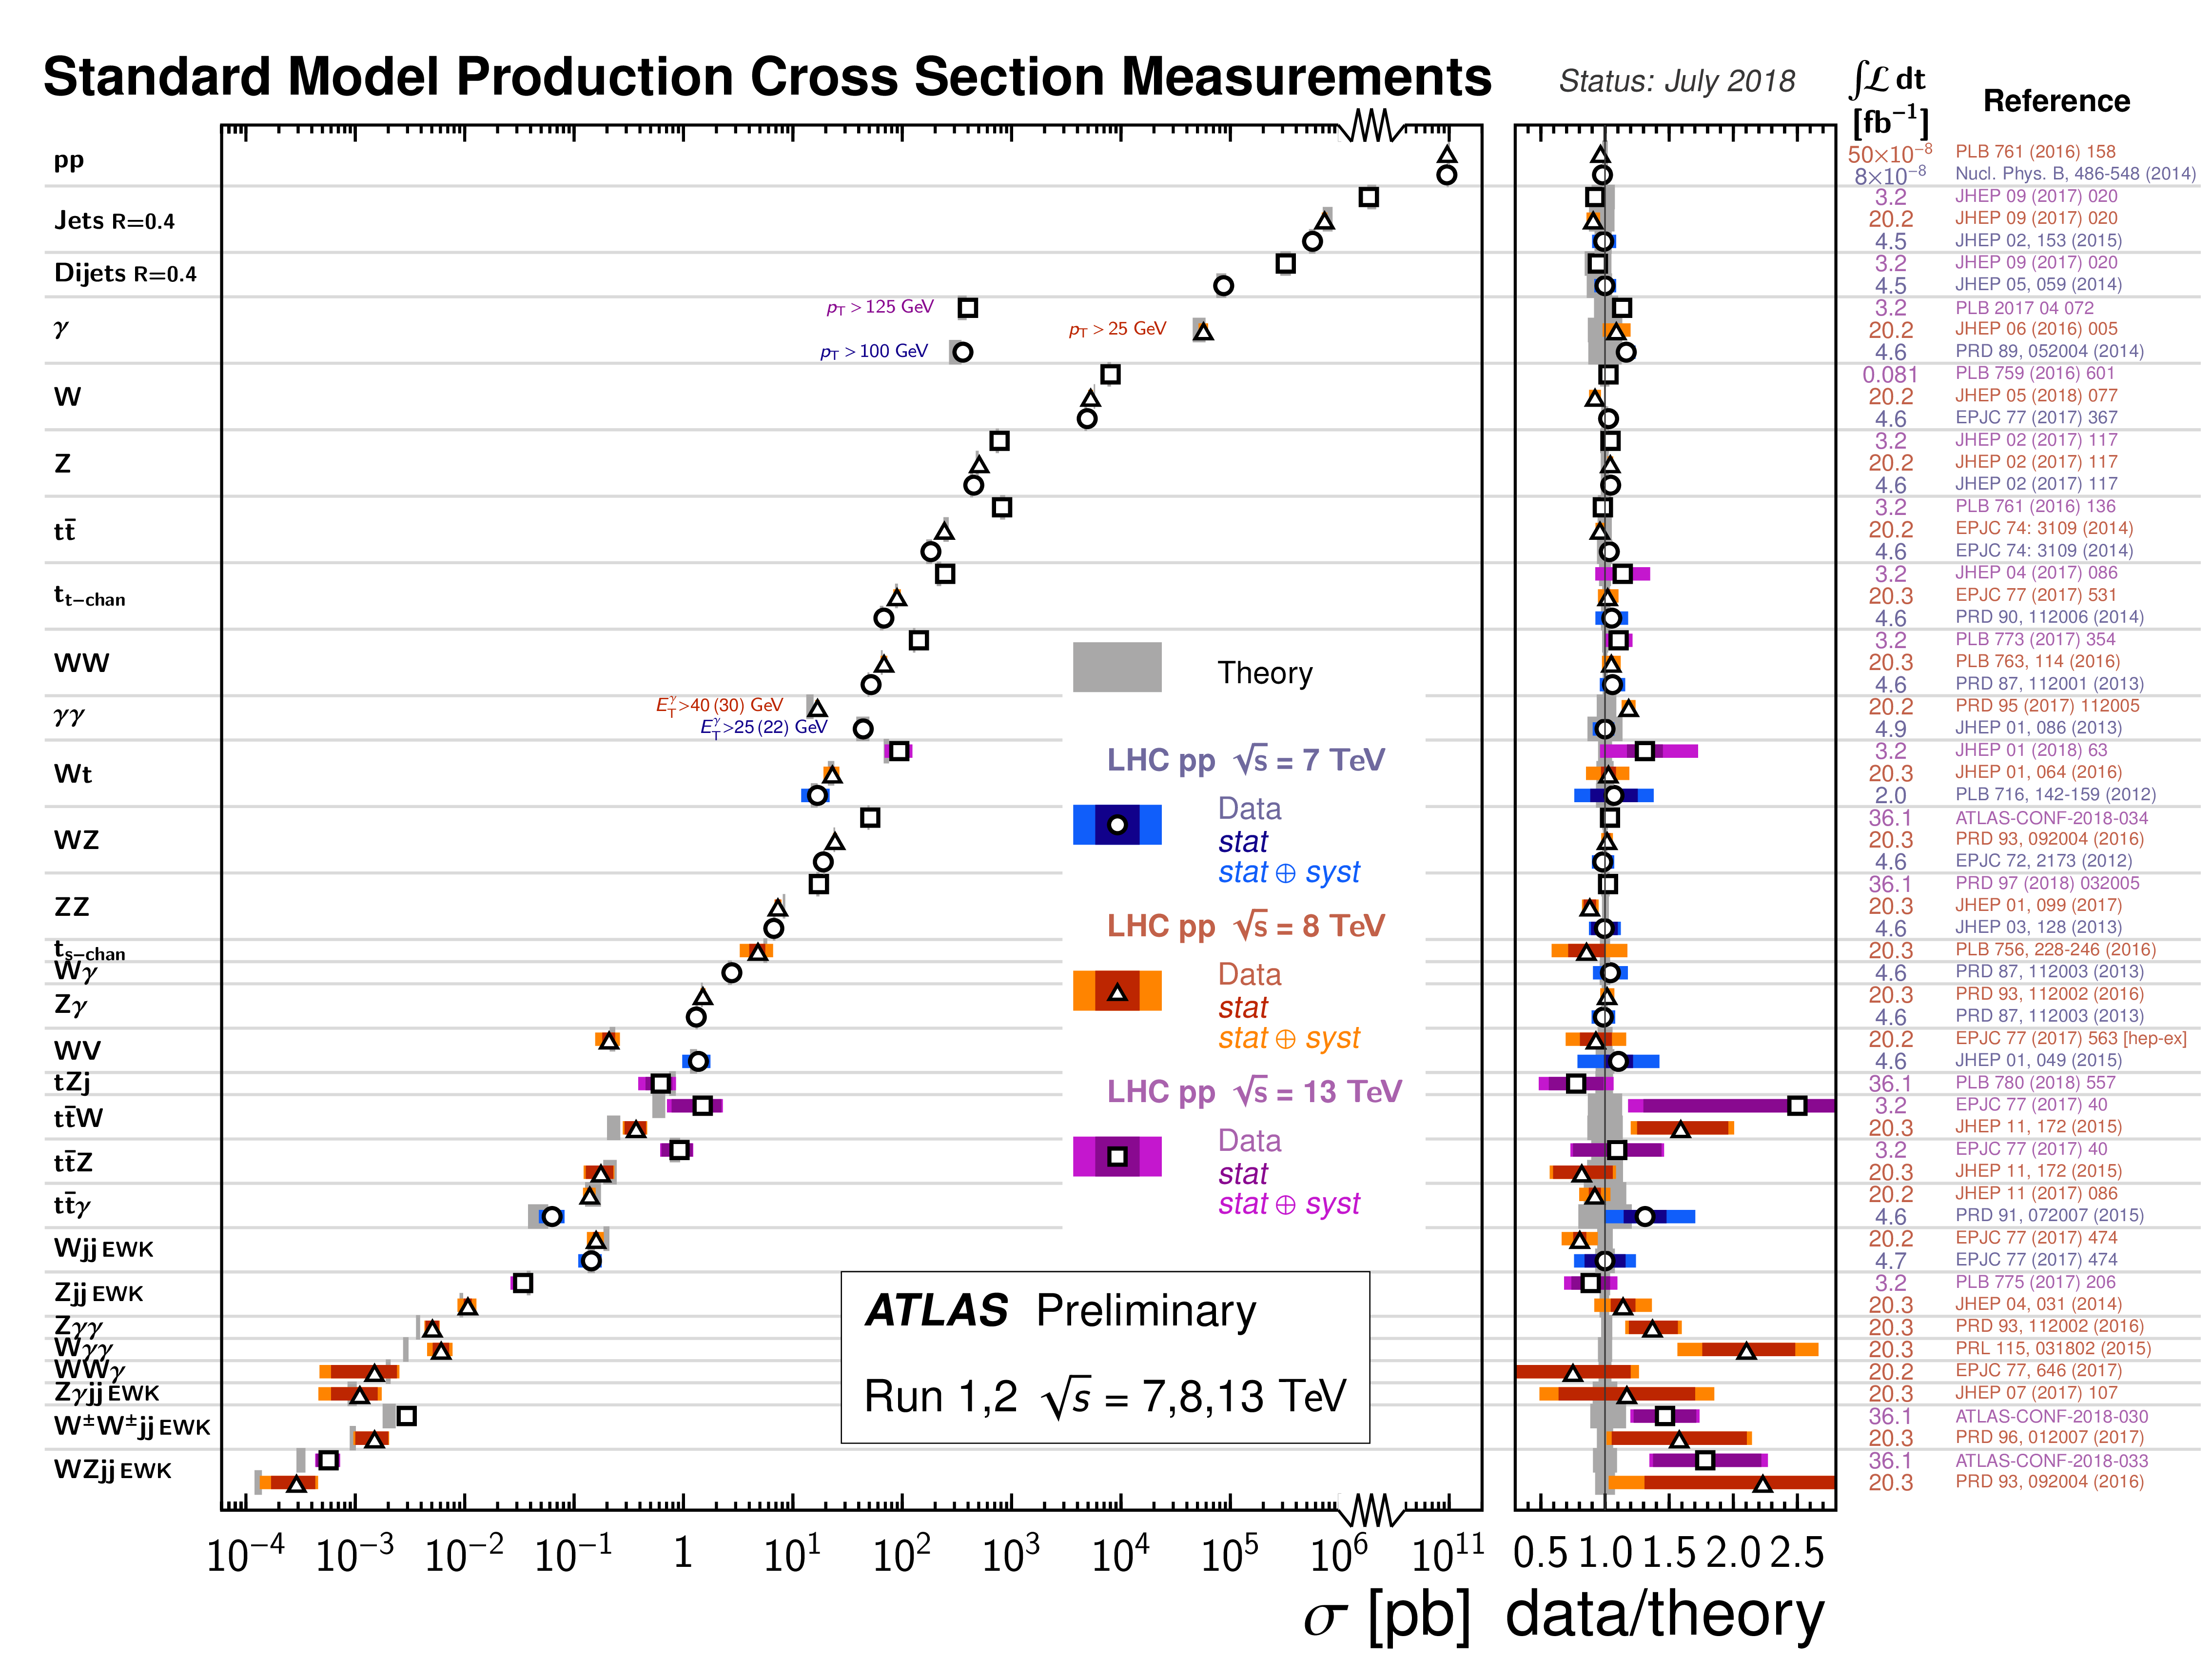
\includegraphics[width=\textwidth,keepaspectratio=true]{ATLAS_d_SMSummary_FiducialXsect_rotated.png}
        % \caption{\tiny}
      \end{figure}
    \end{columns}
  \end{frame}

  \subsection{Supersymmetry }

    \begin{frame}[t]{Supersymmetry}
      \begin{columns}
      \column{.8\textwidth}
        \begin{itemize}
          \item Hierarchy problem, ``unnaturalness''
          \begin{itemize}
            % \item Large Higgs mass terms cancel to give $\sim 125$ GeV
            \item Electroweak scale is $\sim 100$ GeV
            \item Planck scale is $\sim 2.4 \times 10^{18}$ GeV
            \item Supersymmetry (SUSY) offers many new particles to occupy the intermediate range
          \end{itemize}
          \item SUSY proposes a symmetry between fermions and bosons (spin)
          \begin{itemize}
            \item $Q | Fermion \rangle = | Boson \rangle$ 
            \item $Q | Boson \rangle = | Fermion \rangle$
          \end{itemize}
          \item SUSY is a large group of theories
          \begin{itemize}
            \item Minimal Supersymmetric Standard Model (MSSM) is the smallest SUSY extension to the SM
            \item 2 Higgs Doublet Models have two complex doublet scalar fields
            \begin{itemize}
              \item Two relevant free parameters, \tanb and \mHpm
              \item \tanb is the ratio of the vacuum expectation values of \Hpm
            \end{itemize}
          \end{itemize}
        \end{itemize}
      \column{.2\textwidth}
        \begin{table}[!thp]
          \centering
          \resizebox{\textwidth}{!}{
          \begin{tabular}{| l | c |}
          \hline
          light neutral scalar  & $h^0$ \\ \hline
          heavy neutral scalar  & $H^0$ \\ \hline
          neutral pseudoscalar  & $A^0$ \\ \hline
          two charged scalars   & \Hpm \\ \hline
          \end{tabular}}
          % \caption{\cite{2HDM}}
      \end{table}
      \end{columns}
    \end{frame}

  \subsection{Charged Higgs Bosons }

\section{Experimental Apparatus }

  \subsection{LHC }

  \subsection{The ATLAS Detector }

\section{Simulation }

\section{Event Reconstruction }

\section{\HpmLong }
  
  \subsection{Signature }

  \subsection{Event Selection }

  \subsection{Datasets }

  \subsection{Background Modeling }

  \subsection{MVA }

  \subsection{Systematic Uncertainties }

  \subsection{Results }

\section{Conclusion }

  \begin{frame}{Thank You}
    \centering
    \includegraphics[height=7.4cm, keepaspectratio=true]{CERN_globe.jpeg}
  \end{frame}


%%%%%%%%%%%%%%%%%%%%%%%%%%%%%%%%%%%%%%%%%%%%%%%%%%%%%%%%%%%%%%%%%%%%%%%%%%%%%%%%%
%%%%%%%%%%%%%%%%%%%%%%%%%%%%%%%%%%%%%%%%%%%%%%%%%%%%%%%%%%%%%%%%%%%%%%%%%%%%%%%%%
%%%%%%%%%%%%%%%%%%%%%%%%%%%%%%%%%%%%%%%%%%%%%%%%%%%%%%%%%%%%%%%%%%%%%%%%%%%%%%%%%
%%%%%%%%%%%%%%%%%%%%%%%%%%%%%%%%%%%%%%%%%%%%%%%%%%%%%%%%%%%%%%%%%%%%%%%%%%%%%%%%%
\appendix
\section{Bibliography }

  \begin{frame}[allowframebreaks]
          \frametitle{References}
          % \nocite{*}
          % \bibliographystyle{amsalpha}
          \printbibliography
  \end{frame}

\section{Backup }

\end{document}